\section{Durchführung}
\label{sec:Durchführung}

In Abbildung 4 ist die Messapparatur dargestellt.
Mit einem Geiger-Müller-Zählrohr wird die Strahlintensität gemessen.
Ein Zählwerk wird über einen Verstärker angeschlossen und mit Hilfe eines Zeitgebers wird die Messzeit eingestellt.
Die ganze Vorrichung ist von einer Blei-Wand umgeben. 

Bevor die Messung gestartet wird und muss der Nulleffekt bestimmt werden. Dazu wird ohne radioakive Quelle die Zählrate mindestens 900 Sekunden gemessen.
Dann wird die Strahlungsquelle eingesetzt und Beta-und Gamma-Absorptionskurven bestimmt.
Für die Beta-Kurve werden Aluminium-Blöcke unterschiedlicher Dicke in die Apparatur eingesetzt, und bei der ersten dicksten Platte wird für 1100 Sekunden gemessen.
Danach werden immer 100 Sekunden weniger gemessen.
Es werden für Blei und Eisen die  Gamma-Intensitäten bestimmt. Dazu wird ähnlich wie bei der Beta-Strahlung verfahren, es werden unterschiedliche Dicken für unterschiedliche Zeiten untersucht.

\begin{figure}[H]
  \centering
  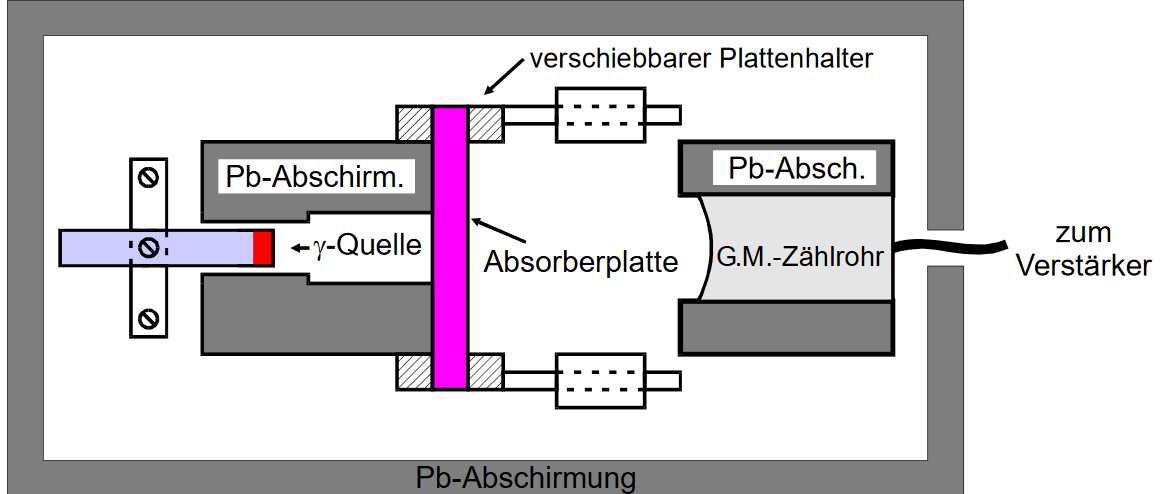
\includegraphics[width=0.8\textwidth]{messapparatur.png}
  \caption{Aufbau der Messapparatur.\cite[S.14]{kent}}
  \label{fig:aufbau}
\end{figure}
